\documentclass[12pt,a4paper]{article}
\usepackage[utf8]{inputenc}
\usepackage[T1]{fontenc}
\usepackage{amsmath}
\usepackage{amsfonts}
\usepackage{amssymb}
\usepackage{graphicx}
\usepackage{hyperref}
\usepackage[polish]{babel}
\usepackage{algorithm}
\usepackage{algpseudocode}
\usepackage{booktabs}
\usepackage{float}

\title{Sprawozdanie z implementacji heurystyk konstrukcyjnych dla zmodyfikowanego problemu komiwojażera}
\author{Filip Rosiak 151799  \and Eryk Stec 152948}
\date{\today}

\begin{document}

\maketitle

\begin{abstract}
W niniejszym sprawozdaniu przedstawiono implementację i analizę heurystyk konstrukcyjnych dla zmodyfikowanego problemu komiwojażera. Problem polega na ułożeniu dwóch rozłącznych zamkniętych ścieżek, każda zawierająca około 50\% wierzchołków, minimalizując łączną długość obu ścieżek. Zaimplementowano i porównano cztery algorytmy: metodę najbliższego sąsiada, metodę rozbudowy cyklu, algorytm UTCU z 2-żalem oraz algorytm z ważonym 2-żalem. Eksperymenty przeprowadzono na instancjach kroa200 i krob200 z biblioteki TSPLib.
\end{abstract}

\section{Opis problemu}
Rozważany problem jest modyfikacją klasycznego problemu komiwojażera. Dany jest zbiór wierzchołków i symetryczna macierz odległości pomiędzy dowolną parą wierzchołków. Zadanie polega na ułożeniu dwóch rozłącznych zamkniętych ścieżek (cykli), każda zawierająca 50\% wierzchołków (jeżeli liczba wierzchołków w instancji nie jest parzysta, to pierwsza ścieżka zawiera jeden wierzchołek więcej), minimalizując łączną długość obu ścieżek.

Do testów wykorzystano instancje \texttt{kroa200} i \texttt{krob200} z biblioteki TSPLib. Są to dwuwymiarowe instancje euklidesowe, gdzie dla każdego wierzchołka podane są dwie współrzędne, a odległość pomiędzy wierzchołkami jest odległością euklidesową zaokrąglaną do liczby całkowitej.

\section{Zaimplementowane algorytmy}
W ramach zadania zaimplementowano następujące heurystyki konstrukcyjne:

\subsection{Algorytm najbliższego sąsiada}
Algorytm jest inspirowany metodą najbliższego sąsiada dla klasycznego problemu komiwojażera, dostosowany do rozważanego problemu z dwoma cyklami.

\begin{algorithm}
\caption{Algorytm najbliższego sąsiada dla zmodyfikowanego problemu komiwojażera}
\begin{algorithmic}[1]
\State \textbf{Znajdź punkty startowe:}
\State Znajdź parę wierzchołków $(s_1, s_2)$ z maksymalną odległością między nimi
\State Te wierzchołki będą punktami startowymi dla cykli $C_1$ i $C_2$

\State \textbf{Rozdziel dostępne wierzchołki:}
\State Usuń $s_1$ i $s_2$ z dostępnych wierzchołków
\State Podziel pozostałe wierzchołki na dwie grupy:
\State $A_1$ = wierzchołki o parzystych indeksach
\State $A_2$ = wierzchołki o nieparzystych indeksach
\State (Zapewnia to równomierny rozkład i niejawne naprzemienne przydzielanie)

\State \textbf{Zbuduj pierwszy cykl ($C_1$):}
\State Zacznij od $s_1$
\While{$|C_1| < \lceil n/2 \rceil$ i $A_1$ nie jest puste}
    \State Znajdź wierzchołek $v$ w $A_1$ najbliższy ostatniemu wierzchołkowi w $C_1$
    \State Dodaj $v$ do $C_1$
    \State Usuń $v$ z $A_1$
\EndWhile

\State \textbf{Zbuduj drugi cykl ($C_2$):}
\State Zacznij od $s_2$
\While{$|C_2| < \lfloor n/2 \rfloor$ i $A_2$ nie jest puste}
    \State Znajdź wierzchołek $v$ w $A_2$ najbliższy ostatniemu wierzchołkowi w $C_2$
    \State Dodaj $v$ do $C_2$
    \State Usuń $v$ z $A_2$
\EndWhile

\State \Return $(C_1, C_2)$
\end{algorithmic}
\end{algorithm}

\subsection{Algorytm rozbudowy cyklu}
Algorytm jest inspirowany metodą rozbudowy cyklu (greedy cycle) dla klasycznego problemu komiwojażera, dostosowany do rozważanego problemu z dwoma cyklami.

\begin{algorithm}
\caption{Algorytm rozbudowy cyklu dla zmodyfikowanego problemu komiwojażera}
\begin{algorithmic}[1]
\State \textbf{Znajdź punkty startowe:}
\State Znajdź parę wierzchołków $(s_1, s_2)$ z maksymalną odległością między nimi
\State Te wierzchołki będą punktami startowymi dla cykli $C_1$ i $C_2$

\State \textbf{Rozdziel dostępne wierzchołki:}
\State Usuń $s_1$ i $s_2$ z dostępnych wierzchołków
\State Podziel pozostałe wierzchołki na dwie grupy:
\State $A_1$ = wierzchołki o parzystych indeksach
\State $A_2$ = wierzchołki o nieparzystych indeksach

\State \textbf{Dla każdego cyklu $C_i$ zaczynającego się od $s_i$:}
\State Inicjalizuj cykl z wierzchołkiem $s_i$
\State Znajdź najbliższy wierzchołek $v$ do $s_i$ w $A_i$
\State Dodaj $v$ do cyklu i usuń z $A_i$
\While{cykl nie osiągnął docelowego rozmiaru i $A_i$ nie jest puste}
    \For{każdy wierzchołek $v$ w $A_i$}
        \State Spróbuj wstawić $v$ między każdą parę kolejnych wierzchołków w cyklu
        \State Oblicz koszt: koszt\_nowych\_krawędzi - koszt\_usuniętej\_krawędzi
    \EndFor
    \State Wybierz wierzchołek i pozycję z minimalnym kosztem wstawienia
    \State Wstaw wybrany wierzchołek na wybranej pozycji
    \State Usuń wierzchołek z $A_i$
\EndWhile

\State \Return $(C_1, C_2)$
\end{algorithmic}
\end{algorithm}

\subsection{Algorytm UTCU z 2-żalem}
Algorytm wykorzystuje koncepcję 2-żalu (2-regret) na bazie algorytmu rozbudowy cyklu.

\begin{algorithm}
\caption{Algorytm UTCU z 2-żalem dla zmodyfikowanego problemu komiwojażera}
\begin{algorithmic}[1]
\State \textbf{Znajdź punkty startowe:}
\State Znajdź parę wierzchołków $(s_1, s_2)$ z maksymalną odległością między nimi
\State Te wierzchołki będą punktami startowymi dla cykli $C_1$ i $C_2$

\State \textbf{Rozdziel dostępne wierzchołki:}
\State Usuń $s_1$ i $s_2$ z dostępnych wierzchołków
\State Podziel pozostałe wierzchołki na dwie grupy:
\State $A_1$ = wierzchołki o parzystych indeksach
\State $A_2$ = wierzchołki o nieparzystych indeksach

\State \textbf{Dla każdego cyklu $C_i$ zaczynającego się od $s_i$:}
\State Inicjalizuj cykl z wierzchołkiem $s_i$
\State Znajdź najbliższy wierzchołek $v$ do $s_i$ w $A_i$
\State Dodaj $v$ do cyklu i usuń z $A_i$
\While{cykl nie osiągnął docelowego rozmiaru i $A_i$ nie jest puste}
    \For{każdy wierzchołek $v$ w $A_i$}
        \State Oblicz koszty dla wszystkich możliwych pozycji wstawienia
        \State Posortuj koszty rosnąco
        \State Oblicz 2-żal jako różnicę między drugim najlepszym a najlepszym kosztem
    \EndFor
    \State Wybierz wierzchołek z największą wartością 2-żalu
    \State Wstaw go w najlepszej pozycji
    \State Usuń wierzchołek z $A_i$
\EndWhile

\State \Return $(C_1, C_2)$
\end{algorithmic}
\end{algorithm}

\subsection{Algorytm z ważonym 2-żalem}
Algorytm łączy koncepcję 2-żalu z regułą zachłanną, stosując wagi dla obu składników.

\begin{algorithm}
\caption{Algorytm z ważonym 2-żalem dla zmodyfikowanego problemu komiwojażera}
\begin{algorithmic}[1]
\State \textbf{Znajdź punkty startowe:}
\State Znajdź parę wierzchołków $(s_1, s_2)$ z maksymalną odległością między nimi
\State Te wierzchołki będą punktami startowymi dla cykli $C_1$ i $C_2$

\State \textbf{Rozdziel dostępne wierzchołki:}
\State Usuń $s_1$ i $s_2$ z dostępnych wierzchołków
\State Podziel pozostałe wierzchołki na dwie grupy:
\State $A_1$ = wierzchołki o parzystych indeksach
\State $A_2$ = wierzchołki o nieparzystych indeksach

\State \textbf{Ustal wagi:} $w_r = 1.0$ (waga dla żalu), $w_g = -1.0$ (waga dla kosztu zachłannego)

\State \textbf{Dla każdego cyklu $C_i$ zaczynającego się od $s_i$:}
\State Inicjalizuj cykl z wierzchołkiem $s_i$
\State Znajdź najbliższy wierzchołek $v$ do $s_i$ w $A_i$
\State Dodaj $v$ do cyklu i usuń z $A_i$
\While{cykl nie osiągnął docelowego rozmiaru i $A_i$ nie jest puste}
    \For{każdy wierzchołek $v$ w $A_i$}
        \State Oblicz koszty dla wszystkich możliwych pozycji wstawienia
        \State Posortuj koszty rosnąco
        \State Oblicz najlepszy koszt wstawienia $c_1(v)$
        \State Oblicz drugi najlepszy koszt wstawienia $c_2(v)$
        \State Oblicz żal: $regret(v) = c_2(v) - c_1(v)$
        \State Oblicz ważoną ocenę: $score(v) = w_r \cdot regret(v) + w_g \cdot c_1(v)$
    \EndFor
    \State Wybierz wierzchołek z najwyższą wartością ważonej oceny
    \State Wstaw go w najlepszej pozycji
    \State Usuń wierzchołek z $A_i$
\EndWhile

\State \Return $(C_1, C_2)$
\end{algorithmic}
\end{algorithm}

\section{Wyniki eksperymentów}
Każdy algorytm został uruchomiony na instancjach kroa200 i krob200. Poniżej przedstawiono wyniki eksperymentów.

\begin{table}[H]
\centering
\caption{Wyniki eksperymentów dla instancji kroa200 i krob200}
\begin{tabular}{lcc}
\toprule
\textbf{Algorytm} & \textbf{kroa200} & \textbf{krob200} \\
\midrule
Najbliższy sąsiad & 59501 & 56024 \\
Rozbudowa cyklu & 52361 & 49942 \\
UTCU z 2-żalem & 45373 & 42995 \\
Ważony 2-żal & 51501 & 46284 \\
\bottomrule
\end{tabular}
\end{table}

\begin{table}[H]
\centering
\caption{Czasy wykonania algorytmów [ms]}
\begin{tabular}{lcc}
\toprule
\textbf{Algorytm} & \textbf{kroa200} & \textbf{krob200} \\
\midrule
Najbliższy sąsiad & 0.00 & 0.00 \\
Rozbudowa cyklu & 2.06 & 2.27 \\
UTCU z 2-żalem & 13.02 & 11.46 \\
Ważony 2-żal & 11.05 & 11.45 \\
\bottomrule
\end{tabular}
\end{table}

\section{Wizualizacje}
Poniżej przedstawiono wizualizacje najlepszych rozwiązań dla każdej kombinacji algorytm/instancja.

\subsection{Instancja kroa200}

\begin{figure}[H]
\centering
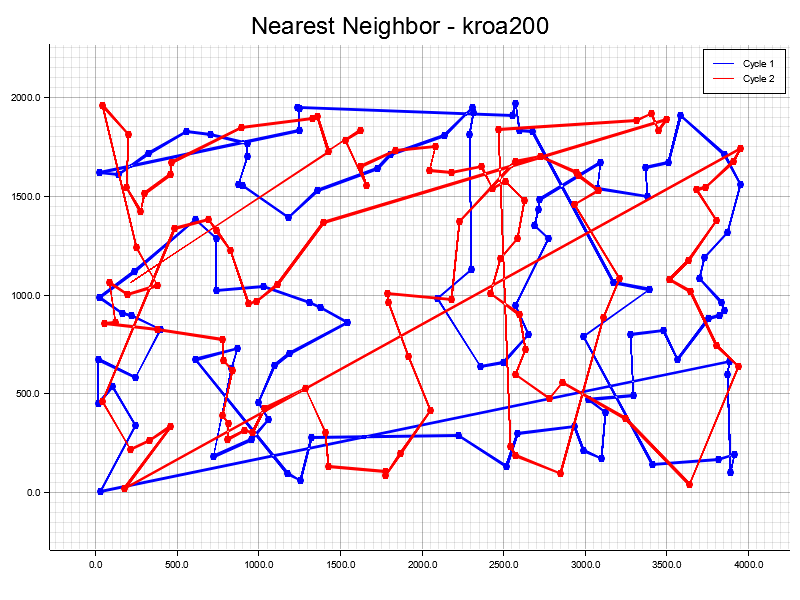
\includegraphics[width=0.8\textwidth]{figures/kroa200_Nearest_Neighbor.png}
\caption{Wizualizacja rozwiązania dla algorytmu najbliższego sąsiada na instancji kroa200}
\end{figure}

\begin{figure}[H]
\centering
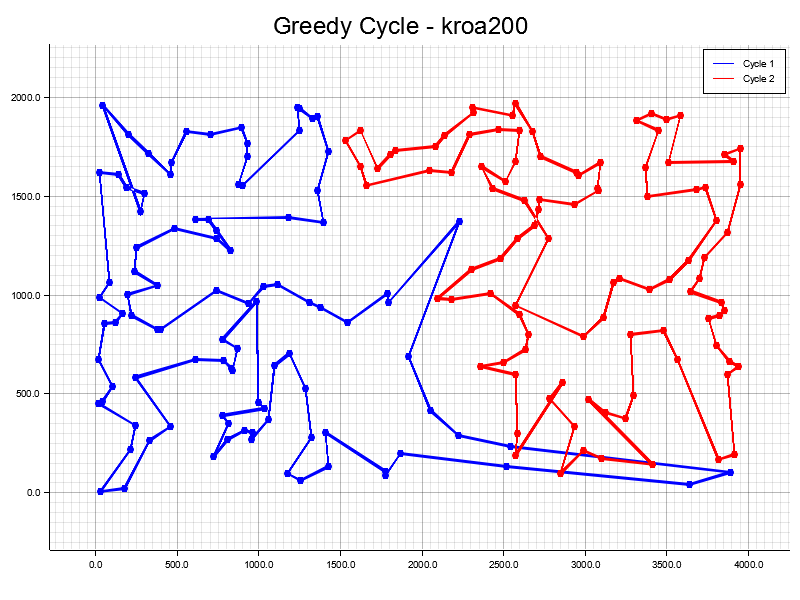
\includegraphics[width=0.8\textwidth]{figures/kroa200_Greedy_Cycle.png}
\caption{Wizualizacja rozwiązania dla algorytmu rozbudowy cyklu na instancji kroa200}
\end{figure}

\begin{figure}[H]
\centering
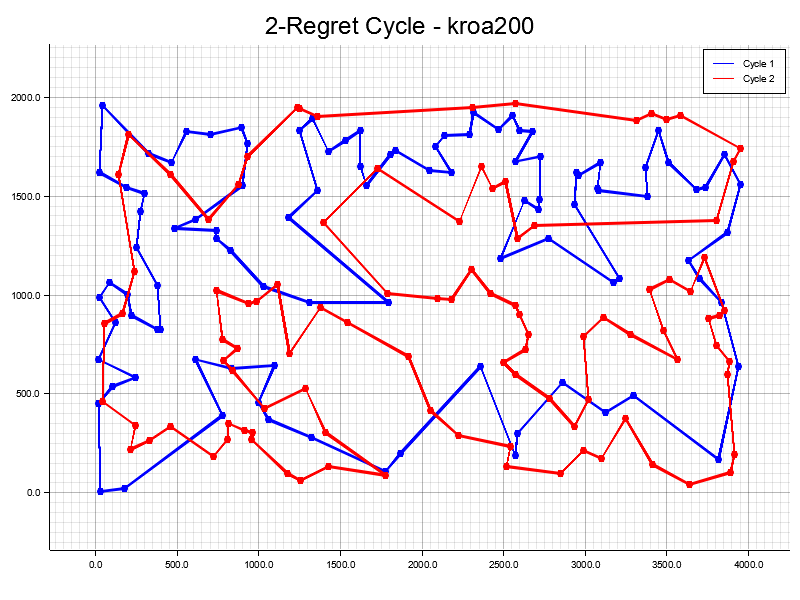
\includegraphics[width=0.8\textwidth]{figures/kroa200_2-Regret_Cycle.png}
\caption{Wizualizacja rozwiązania dla algorytmu UTCU z 2-żalem na instancji kroa200}
\end{figure}

\begin{figure}[H]
\centering
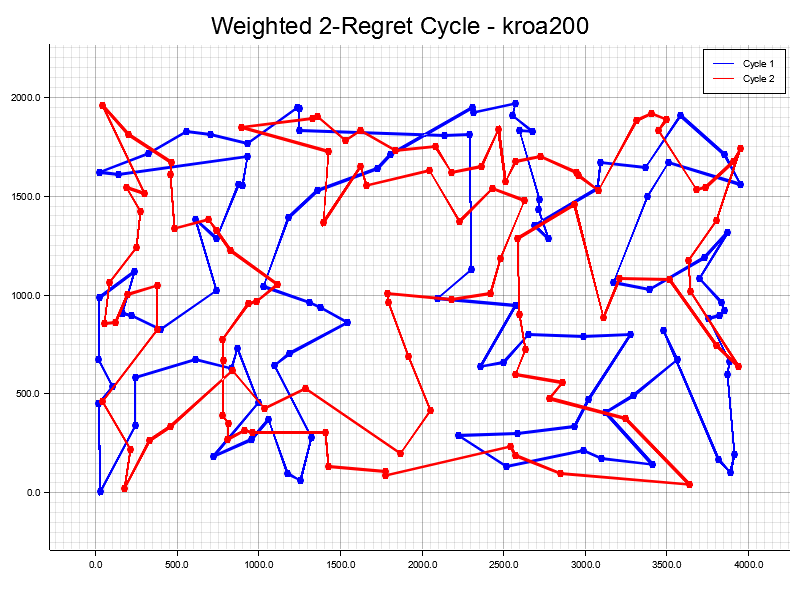
\includegraphics[width=0.8\textwidth]{figures/kroa200_Weighted_2-Regret_Cycle.png}
\caption{Wizualizacja rozwiązania dla algorytmu z ważonym 2-żalem na instancji kroa200}
\end{figure}

\subsection{Instancja krob200}

\begin{figure}[H]
\centering
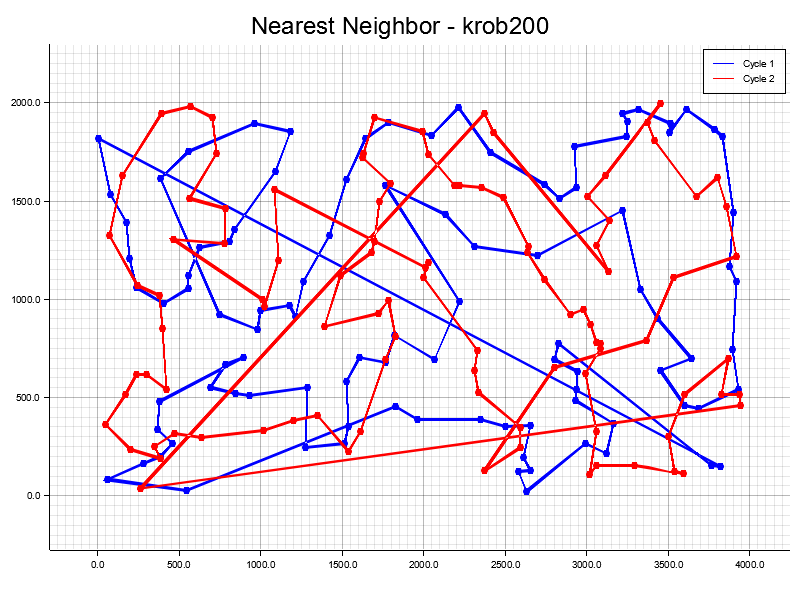
\includegraphics[width=0.8\textwidth]{figures/krob200_Nearest_Neighbor.png}
\caption{Wizualizacja rozwiązania dla algorytmu najbliższego sąsiada na instancji krob200}
\end{figure}

\begin{figure}[H]
\centering
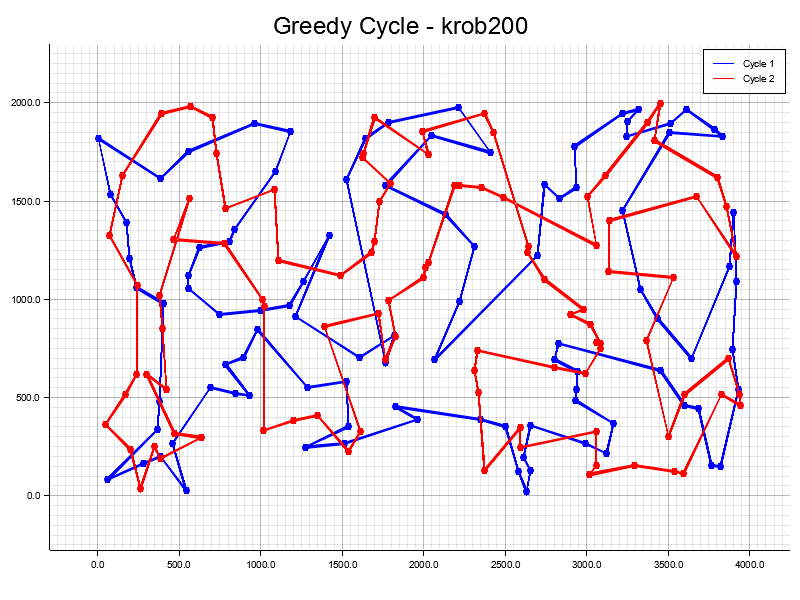
\includegraphics[width=0.8\textwidth]{figures/krob200_Greedy_Cycle.png}
\caption{Wizualizacja rozwiązania dla algorytmu rozbudowy cyklu na instancji krob200}
\end{figure}

\begin{figure}[H]
\centering
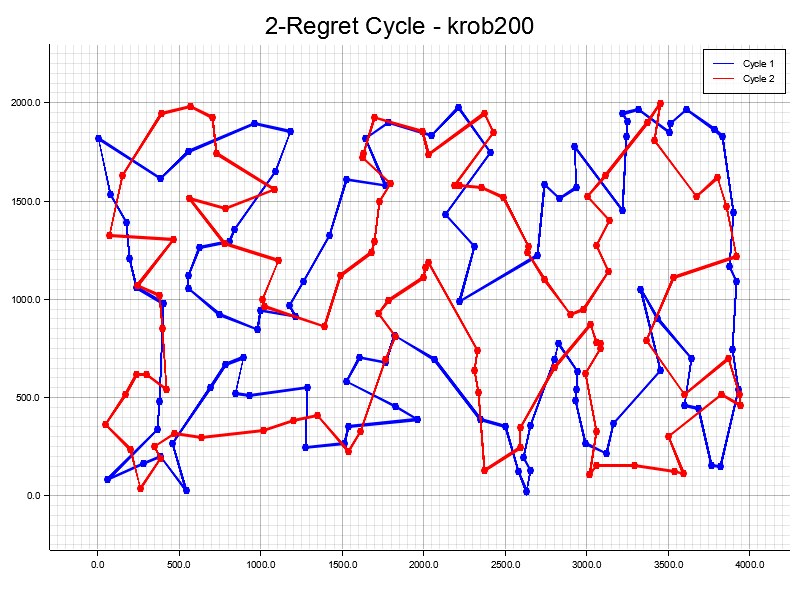
\includegraphics[width=0.8\textwidth]{figures/krob200_2-Regret_Cycle.png}
\caption{Wizualizacja rozwiązania dla algorytmu UTCU z 2-żalem na instancji krob200}
\end{figure}

\begin{figure}[H]
\centering
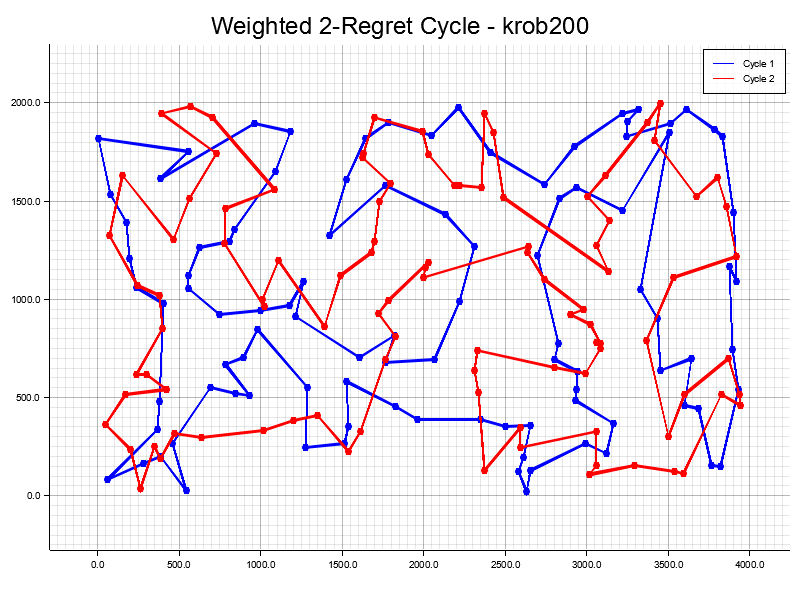
\includegraphics[width=0.8\textwidth]{figures/krob200_Weighted_2-Regret_Cycle.png}
\caption{Wizualizacja rozwiązania dla algorytmu z ważonym 2-żalem na instancji krob200}
\end{figure}

\section{Wnioski}
Na podstawie przeprowadzonych eksperymentów można wyciągnąć następujące wnioski:

\begin{enumerate}
    \item Algorytm UTCU z 2-żalem osiągnął najlepsze wyniki dla obu instancji, uzyskując najniższe koszty rozwiązań (45373 dla kroa200 i 42995 dla krob200).
    
    \item Algorytm najbliższego sąsiada, mimo że jest najszybszy (czas wykonania bliski 0 ms), daje najgorsze wyniki pod względem jakości rozwiązań (59501 dla kroa200 i 56024 dla krob200).
    
    \item Algorytm rozbudowy cyklu oferuje dobry kompromis między jakością rozwiązania a czasem wykonania, osiągając wyniki lepsze niż algorytm najbliższego sąsiada przy niewielkim koszcie czasowym (około 2 ms).
    
    \item Algorytm z ważonym 2-żalem, mimo podobnego czasu wykonania jak UTCU z 2-żalem, daje gorsze wyniki. Może to sugerować, że zastosowane wagi ($w_r = 1.0$, $w_g = -1.0$) nie są optymalne dla rozważanego problemu.
    
    \item Wszystkie algorytmy oparte na żalu (UTCU z 2-żalem i ważony 2-żal) wymagają znacznie więcej czasu obliczeniowego niż prostsze heurystyki, co jest spowodowane koniecznością obliczania i porównywania kosztów dla wszystkich możliwych pozycji wstawienia.
    
    \item Wizualizacje rozwiązań pokazują, że algorytmy oparte na żalu tworzą bardziej regularne i krótsze cykle, podczas gdy algorytm najbliższego sąsiada tworzy cykle z większą liczbą przecięć i dłuższych krawędzi.
\end{enumerate}

Podsumowując, wybór odpowiedniego algorytmu zależy od priorytetów: jeśli najważniejsza jest jakość rozwiązania, należy wybrać algorytm UTCU z 2-żalem; jeśli czas wykonania jest krytyczny, algorytm najbliższego sąsiada będzie najlepszym wyborem; natomiast algorytm rozbudowy cyklu stanowi rozsądny kompromis między jakością a czasem wykonania.

\section{Kod źródłowy}
Pełny kod źródłowy implementacji wszystkich algorytmów jest dostępny w repozytorium GitHub:
\url{https://github.com/Veanir/imo-1}

\end{document} 